\NeedRoom{10}

\subsection{Financial Sensitivity}

\begin{figure}[htbp]\centering

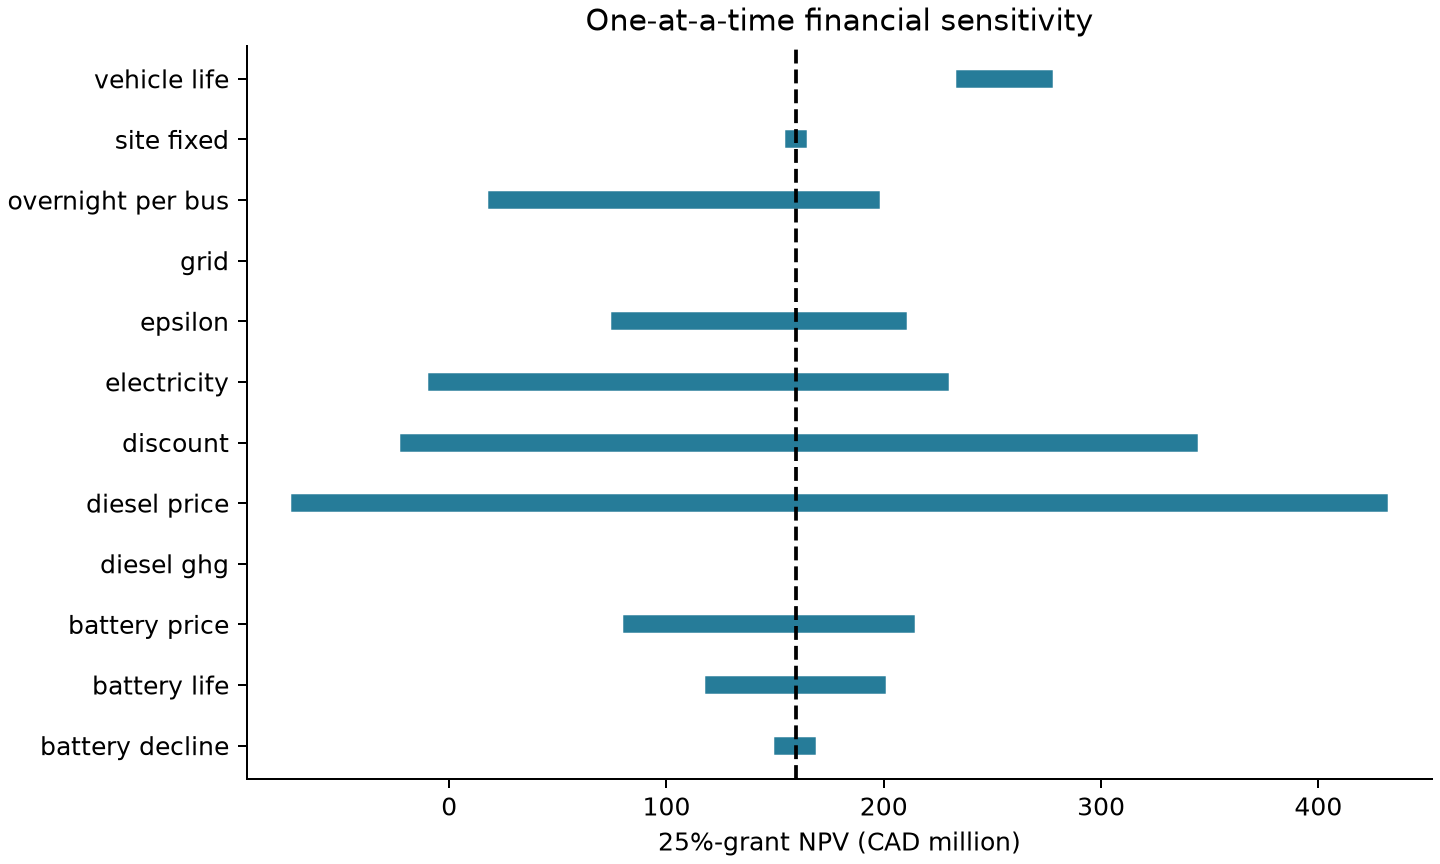
\includegraphics[width=\textwidth,height=0.37\textheight,keepaspectratio]{images/tornado.png}

\caption{One-at-a-time 25\%-grant NPV sensitivity; dashed line is the central scenario.}\label{fig:result3}

\end{figure}

The parameter ledger distinguishes primary observations, historical transfers and explicit assumptions. Energy and diesel prices, battery cost and learning, discount rate, lives, infrastructure allowances and baseline fuels are varied. R/T cases also recompute the operating schedule, rather than imposing a new battery cost on a frozen fleet.


The all-in electricity price is a screening allowance, not an hourly tariff model. In particular, a historically temporary zero-demand tariff is not extended through 2033. Local interconnection quotes, construction schedules and body-specific costs are still missing.


A fossil-diesel counterfactual can overstate the benefit relative to continued low-carbon fuels. High grants can improve the agency balance while total resource cost remains higher. Those distinct questions should not be hidden in an unexplained weighted score.


A deliberately optimistic diesel cost bound removes all diesel deadhead while retaining the same fleet. The 25\%-grant NPV then falls to CAD 0.5 million. The central financial result therefore depends materially on the diesel assignment, which minimizes fleet size rather than travel cost.

